\documentclass{article}
    \usepackage{amssymb}
    \usepackage[utf8]{inputenc}
    \usepackage[russian]{babel}
    \usepackage[left=2cm,right=2cm,
        top=2cm,bottom=2cm,bindingoffset=0cm]{geometry}
    \usepackage{hyperref}
    \hypersetup{
        colorlinks=true,
        linkcolor=blue,
        filecolor=magenta,      
        urlcolor=cyan,
    }
  \usepackage{graphicx}
  \graphicspath{{pictures/}}
  \DeclareGraphicsExtensions{.pdf,.png,.jpg}

\begin{document}
\begin{center}{\hugeОтчет по курсовой работе за неделю\\}\end{center}
Дата: 8.10.2020\\
Научные руководители: Герасимов С.В., Мещеряков А.В.\\
Студент: Немешаева Алиса\\
Курс: 4\\

\renewcommand{\labelitemi}{$\blacksquare$}
\renewcommand\labelitemii{$\square$}
\begin{enumerate}
    \item На этой неделе проводилось исследование различных нейросетевых архитектур, которые могут
        улучшить результаты существующих моделей.\\
    \item Были изучены следующие модели:\\
        \begin{itemize}
            \item \hyperlink{https://arxiv.org/pdf/1612.01105.pdf}{PSPNet}\\ 
            \item \hyperlink{https://arxiv.org/pdf/1707.03718.pdf}{LinkNet}\\
            \item \hyperlink{https://arxiv.org/pdf/2009.01907.pdf}{W-Net}\\
        \end{itemize}
    \item На базе обученной ранее модели были созданы каталоги с детектированными скоплениями 
        галактик.\\

\end{enumerate}

\begin{figure}[h]
    \begin{minipage}[h]{0.47\linewidth}
        \center{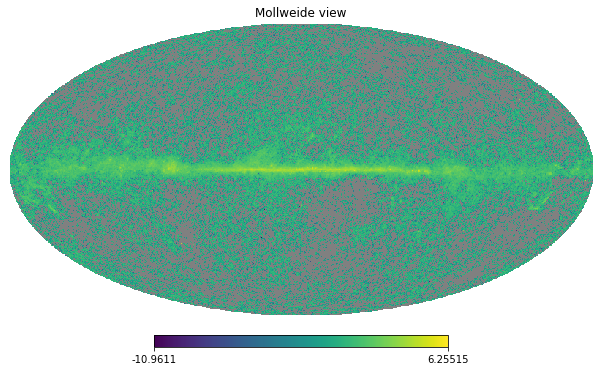
\includegraphics[width=1\linewidth]{100}} 100 \\
    \end{minipage}
\hfill
    \begin{minipage}[h]{0.47\linewidth}
        \center{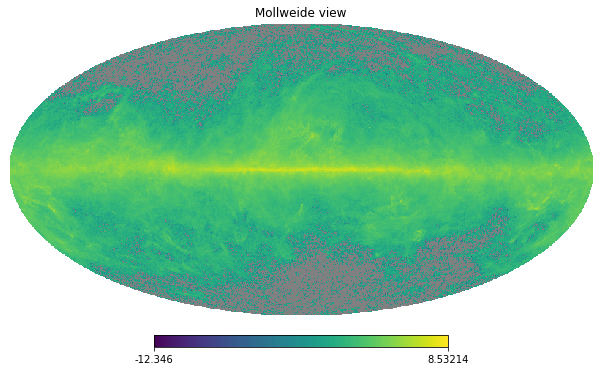
\includegraphics[width=1\linewidth]{353}} \\353
    \end{minipage}
\vfill
    \begin{minipage}[h]{0.47\linewidth}
        \center{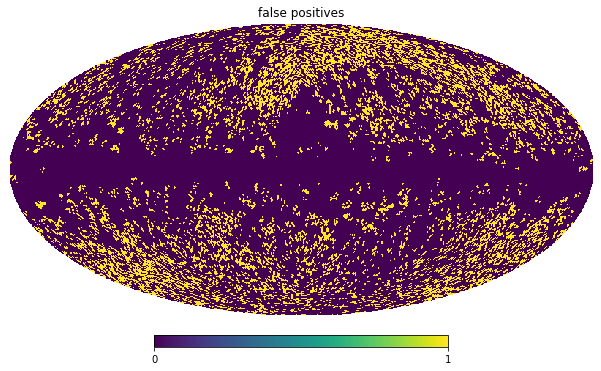
\includegraphics[width=1\linewidth]{fp}} false positives \\
    \end{minipage}
\hfill
    \begin{minipage}[h]{0.47\linewidth}
        \center{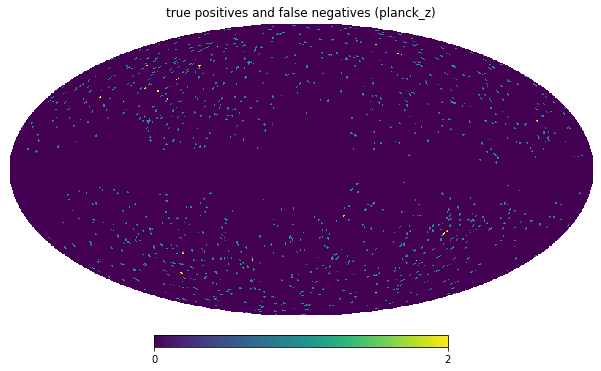
\includegraphics[width=1\linewidth]{planck_z}} planck\_z \\
    \end{minipage}
    \caption{Сигнал микроволновых данных Planck по двум каналам 100 и 353. (Данные, на которых
        проводилась детекция) и карта каталога с результатами сканирования всего неба для модели 
        на 14 эпох с порогом 0.4 для маски сегментации: false positives (объекты, не найденные в 
        выбранных каталогах) и true positives / false negatives для каталога planck\_z, на данных 
        которого обучалась модель}
\end{figure}
На изображении каталога planck\_z синие точки соответствуют true positives, жёлтые - false 
negatives. Общий recall для этой конфигурации для этого каталога составил 0.785 (по всей области 
неба).\\
Общее количество строк кода за эту неделю: 63\\
\end{document}
